\documentclass[table,aspectratio=1610]{beamer}

% ===============================================
%          beamer slides setting
%
%   Author      : Bei Yu
%   Last Update : 16/2018
% ===============================================

\setbeamerfont{frametitle}{size=\LARGE}
\renewcommand{\thefootnote}{\fnsymbol{footnote}}

% =============================================
%            Specify colors
% =============================================
%\usepackage{xcolor}
\definecolor{myorange}{RGB}{244,106,18} %F47012
\definecolor{myblue}{RGB}{0,111,190}    %006FBE
\definecolor{mygreen}{RGB}{0,127,128}   %007F80
\definecolor{myred}{RGB}{228,46,36}     %E42E24
\definecolor{myyellow}{RGB}{198,148,34} %C69422
\definecolor{mydark}{RGB}{114,44,114}   %722C72
\definecolor{mymiddle}{RGB}{144,44,144} %902C90
\definecolor{mylight}{RGB}{167,44,167}  %A72CA7
\definecolor{CUHKorange}{RGB}{244,106,18} %F47012
\definecolor{CUHKblue}{RGB}{0,111,190}    %006FBE
\definecolor{CUHKgreen}{RGB}{0,127,128}   %007F80
\definecolor{CUHKred}{RGB}{228,46,36}     %E42E24
\definecolor{CUHKyellow}{RGB}{198,148,34} %C69422
\definecolor{CUHKdark}{RGB}{114,44,114}   %722C72
\definecolor{CUHKmiddle}{RGB}{144,44,144} %902C90
\definecolor{CUHKlight}{RGB}{167,44,167}  %A72CA7
\setbeamercolor{structure}{fg=CUHKblue}
\setbeamercolor{alerted text}{fg=CUHKorange}

% ==== packages
\usepackage{bm}
\usepackage{algpseudocode}           % for algorithm
\usepackage{algorithm}
\usepackage{pgfpages}                % allow note printing
\usepackage{pgf,pgfarrows,pgfnodes,pgfautomata,pgfheaps,pgfshade}
\usepackage{amsmath}
\usepackage{newtxtext}               % to use Times font (only for text, but not for math)
\usepackage{multirow}
\usepackage{subfig}
\usepackage{filecontents}
\usepackage{pgfplots}
\usepackage{graphicx}
\usepackage{caption}
\usepackage{tikz}
\usepackage{tikzscale}
%\captionsetup[figure]{font=scriptsize,textfont={color=CUHKgreen},labelformat=empty}
\captionsetup[figure]{font=footnotesize,labelformat=empty}
\usepackage[english]{babel}
\usepackage{wasysym}                 % smiling face
\usepackage{animate}                 % animation 
\usefonttheme[onlymath]{serif}       % 
\usepackage{etoolbox}                % commands \newtoggle, \toggletrue, \iftoggle
\usepackage{courier}                 % courier font, used in \texttt
\usepackage{soul}
\usepackage{booktabs}                % toprule bottomrule
\usepackage{listings}                % typeset source code listings
\lstset{basicstyle=\ttfamily,breaklines=true}
\lstdefinestyle{base}
{
    language   = C,
    emptylines = 1,
    breaklines = true,
    basicstyle = \ttfamily\scriptsize,
    moredelim  = **[is][\color{red}]{@}{@},
}
\usepackage{hyperref}
\hypersetup{
    colorlinks = true,
    urlcolor   = CUHKgreen,
    citecolor  = cyan,
    linkcolor  = CUHKgreen,
}


% =============================================
%         Specify some local functions
% =============================================
\newcommand{\m}[1]{\mathbf{#1}}


% Fix caption package bug
% https://tex.stackexchange.com/questions/426088/texlive-pretest-2018-beamer-and-subfig-collide
\makeatletter
\let\@@magyar@captionfix\relax
\makeatother


% Fix UTF-8 encoding problem
% https://tex.stackexchange.com/questions/429190/package-inputenc-error-invalid-utf-8-byte-147
\UseRawInputEncoding

% ======================================================
%             Slides theme
% ======================================================
\mode<presentation> {
  % === background
  %\setbeamertemplate{background canvas}[vertical shading][bottom=red!10,top=blue!10]

  % === setting theme
  %\usetheme{Pittsburgh}
  %\usetheme{Warsaw}         % most complex header
  \usetheme{default}        % only header line
  %\usetheme{Madrid}         % header line and bxottom line
  %\usetheme{AnnArbor}       % simple outline
  %\usefonttheme[onlysmall]{structurebold}
}


% =========================================================
%               Color theme
% =========================================================
%\usecolortheme{wolverine}      % yellow + orange
%\usecolortheme{crane}          % all orange
%\usecolortheme{seahorse}       % blue + grey
\usecolortheme{rose}           % default blue
%\usecolortheme{default}


%\mode<article> % only for the article version
%{
%  \usepackage{fullpage}
%  \usepackage{hyperref}
%}


% ========================================
%           block setting
% ========================================
% varblock
\newenvironment<>{varblock}[2][\textwidth]{%
  \setlength{\textwidth}{#1}
  \setbeamercolor{block title}{fg=white,bg=CUHKblue}
  \setbeamercolor{block body}{fg=black,bg=blue!10}
  \begin{actionenv}#3%
  \def\insertblocktitle{#2}%
  \par%
  \usebeamertemplate{block begin}}
  {
    \par%
    \usebeamertemplate{block end}%
    \end{actionenv}
  }
% question block 
\newenvironment<>{qblock}[2][\textwidth]{%
  \setlength{\textwidth}{#1}
  \setbeamercolor{block title}{fg=black,bg=CUHKyellow!40}
  \setbeamercolor{block body}{fg=black,bg=white}
  \begin{actionenv}#3%
  \def\insertblocktitle{#2}%
  \par%
  \usebeamertemplate{block begin}}
  {
    \par%
    \usebeamertemplate{block end}%
    \end{actionenv}
  }
\setbeamerfont{block title}{size=\large}
\setbeamerfont{block title example}{size=\large}
\setbeamerfont{block title alerted}{size=\large}
\setbeamercolor{block title}{fg=CUHKorange}
\setbeamercolor{block title alerted}{fg=CUHKblue}


% ==================================================
%         Corner logo on title page
% ==================================================
%\titlegraphic{
%    \hspace{8cm}
%    \includegraphics[width=1cm]{./figs/logo_utece}
%}

% ==================================================
%              Corner logo
% ==================================================
%\pgfdeclareimage[width=1cm]{logo}{./figs/logo_utda}
%\logo{\vbox{
%\hbox to 1cm{
% \hfil\pgfuseimage{logo}}
%  %\vskip0.1cm
%  %\hbox{\pgfuseimage{ur-logo}}
%  }
%}





% =========================================================
%               Showing page number
% =========================================================
\iftrue
\defbeamertemplate*{footline}{shadow theme}
{
  \leavevmode
  \hbox{\begin{beamercolorbox}[wd=.5\paperwidth,ht=2.5ex,dp=1.125ex,leftskip=.3cm plus1fil,rightskip=.3cm]{author in head/foot}
    \usebeamerfont{author in head/foot}\insertframenumber\,/\,\inserttotalframenumber\hfill\insertshortauthor
  \end{beamercolorbox}
  \begin{beamercolorbox}[wd=.5\paperwidth,ht=2.5ex,dp=1.125ex,leftskip=.3cm,rightskip=.3cm plus1fil]{title in head/foot}
    \usebeamerfont{title in head/foot}\insertshorttitle
  \end{beamercolorbox}}
  \vskip0pt
}
\fi

%\setbeamercovered{dynamic}
%\beamertemplateshadingbackground{white}{white}

% ==== Log
%
%  06/2016: fix bug from caption package
%  11/2016: block settings
%  10/2016: title font size huge -> LARGE
%  09/2016: qblock for teaching slides
%  05/2016: set frametitle size to huge, by default beamer uses 9pt
%  05/2016: customize figure caption: font size, font color, and remove 'Figure' label
%  03/2016: listing, hyperref
%  03/2015: no logo settings in library file, move to local specific tex file 
%  03/2015: package{etoolbox}
%  02/2015: no corner logo in main pages
%  05/2014: new varblock definition;  package{wasysym} to show smiling face
%  10.2014: package{serif} for article style math fonts
%  



\graphicspath{{./figs/}}

% ==== define xmark
\usepackage{pifont}
\newcommand{\xmark}{\ding{56}}
\newcommand{\calC}{\mathcal{C}}
\newcommand{\calD}{\mathcal{D}}
\newcommand{\calO}{\mathcal{O}}
\newcommand{\calP}{\mathcal{P}}
\newcommand{\calNP}{\mathcal{NP}}
\newcommand{\norm}[1]{\left\lVert#1\right\rVert}           % norm of vector and matrix
\definecolor{mygreen2}{RGB}{76,153,0}
\definecolor{mygrey}{RGB}{192,192,192}
\definecolor{myblue2}{RGB}{51,153,255}

% =============================================
%           pre-definitions
% =============================================
\newtoggle{animation}       \togglefalse{animation}
\newtoggle{use-note}        \togglefalse{use-note}
\newtoggle{show-detail}     \toggletrue{show-detail}

% =============================================
%               Set Up Notes
% =============================================
\iftoggle{use-note}
{
%\setbeameroption{show notes on second screen=right}
\setbeameroption{show notes on second screen=bottom}
\setbeamertemplate{note page}[plain] 
}


\title[]{\LARGE\textbf{
    Reinforcement Learning: function approximation
}}
\author[]{\large
  Zihao DENG\\ Wenqian ZHAO
}
\institute{\large
  \textcolor{CUHKgreen}{
  Department of Computer Science and Engineering \\
  The Chinese University of Hong Kong
  }
}
\date{}


% ==================================================
%             logo on title page
% ==================================================
%\titlegraphic
%{
%    \includegraphics[height=1.2cm]{logo-cuhk}
%}



\begin{document}

\usebackgroundtemplate
{
    
\includegraphics[width=\paperwidth,height=\paperheight]{figs/background-1610}
}
\begin{frame}
    \vspace{.2in}
    \titlepage
\end{frame}
\usebackgroundtemplate{}


% ==== Corner logo on each pages
\pgfdeclareimage[width=.8cm]{logo}{./figs/logo-cuhk-sim}
\logo{\vbox{
    \hbox to 1.0cm{
    \hfil\pgfuseimage{logo}}
    }
}
\graphicspath{{./figs/repo/}{./figs/}}
\section{Optical Proximity Correction (OPC)}

%zhaowenqian
\begin{frame}{Markov Decision Process}
    \begin{itemize}
        
        \item The MDP gives us a precise formulation of the environment, given a state st we select an action at and observe $s_{t+1}$ and $r_{t}$ according to the transition probabilities P:\\
        \bigskip
        \hspace{0.5cm}$\bullet$  $S$ - set of possible states \\
        \hspace{0.5cm}$\bullet$  $s_{t}\in S$ - state at step $t$ \\
        \hspace{0.5cm}$\bullet$  $A$ - set of possible actions \\
        \hspace{0.5cm}$\bullet$  $a_{t}\in A$ - selected action at step $t$\\
        \hspace{0.5cm}$\bullet$  $R$ - Reward function. The reward at step $t$ is given by $r_{t+1} = R(s_{t}, a_{t}, s_{t+1})$\\
        \hspace{0.5cm}$\bullet$ $P$ - transition probabilities such that $s_{t+1} ∼ P(s|s_{t},a_{t})$, i.e. \\
        \hspace{0.5cm}$\bullet$  $\rho$ - Initial state distribution such that $s_{0} ∼ \rho(s)$\\
        \bigskip
        \item Agent is defined with a policy function $\pi(a|s)$, mapping from states to actions and can be either deterministic or non-deterministic
        
    \end{itemize}
\end{frame}

\begin{frame}{Markov Decision Process}
    \begin{itemize}
        \item Given an MDP and a policy, an episode can be produced by repeating of:\\

        \hspace{0.5cm}$\bullet$  $a_{t} ∼ \pi(a|s_{t})$\\
        \hspace{0.5cm}$\bullet$  $s_{t+1} ∼P(s|s_{t},a_{t})$ \\
        \hspace{0.5cm}$\bullet$  $r_{t+1} =r(s_{t},a_{t},s_{t+1})$ \\  
        \item which produce:\\
            \begin{center}
                episode $:= s_{0},a_{0},r_{1},s_{1},a_{1},r_{1},...,s_{\tau−1},a_{\tau−1},r_{\tau−1},s_{\tau}$
            \end{center}
        \bigskip
        \item Optimal Solution gives: \\
            \begin{equation}
                \max\limits_{\pi} E [\sum_{t=1}^{\tau} r_{t}]
            \end{equation}
        
    \end{itemize}
\end{frame}


\begin{frame}{Markov Decision Process}
    \begin{itemize}
        \item Value function defined as :
            \begin{equation}
                V^{\pi}(s)=E_{\pi} [\sum_{t=1}^{\tau} r_{t}|s_{0}=s]
            \end{equation}
            \begin{equation}
                V^*(s)=\max\limits_{\pi} E_{\pi} [\sum_{t=1}^{\tau} r_{t}|s_{0}=s]
            \end{equation}
        \item Bellman equation: A recursive relation for value function:
            \begin{equation}
                V^*(s)=\max\limits_{a\in A} E [r_{t+1}+V^*_{s_{t+1}}|s_{t}=s,a_{t}=t]
            \end{equation}
        \item $(TV)(s)$ is the Bellman operator and we can recursively calculate it and update $V(s)$ (value iteration) to reach optimal (Monotonicity and Contraction mapping)
            \begin{equation}
                (TV)(s)=\max\limits_{a\in A} E [r_{t+1}+V^*_{s_{t+1}}|s_{t}=s,a_{t}=t]
            \end{equation}
            \begin{equation}
            V_{k+1}=TV_{k}
            \end{equation}
        \item policy iteration use the same idea, but instead of updating value function, it update Policy $\pi$

        
    \end{itemize}
\end{frame}


\begin{frame}{Markov Decision Process}
    \begin{itemize}
        \item Another approach: State-Value Function: define a quantity $Q: S \times A\rightarrow \mathbb{R}$:\\
        \begin{equation}
        Q^\pi(s,a)=\bar{R}(s,a)+\sum_{s' \in S}^{T} P_{s,a} (s')V^\pi(s')
        \end{equation}
        \item  Recursively Calculate optimal by using Bellman Operator:
        \bigskip
        
        \hspace{0.5cm}$\bullet$ $ FQ(s,a)=\bar{R}(s,a)+\sum_{s' \in S}^{T} P_{s,a} (s') \max\limits_{a'\in A} Q (s',a') $\\
        \hspace{0.5cm}$\bullet$  $Q(s,a)=FQ(s,a)$
        \bigskip
        
        \item Greedy action selection is simple:
        \begin{equation}
        \pi(s)=\arg\max\limits_{a' \in A}Q(s_{t+1},a')
        \end{equation}
    \end{itemize}
\end{frame}


\begin{frame}{MDP vs RL}
    \begin{itemize}
        \item Difference between Markov Decision Process and Reinforcement learning:\\
        \bigskip
        \hspace{0.5cm}$\bullet$  MDP: the transition matrix $P(s'|s,a)$ is known $\rightarrow$ used to find the optimal agent\\
        \hspace{0.5cm}$\bullet$  RL: $P(s'|s,a)$ unknown and need to be learned :\\
        \hspace{1cm}\romannumeral1 . Iteracting with environment \\
        \hspace{1cm}\romannumeral2 . Requiring explicit knowledge of $P$
        \bigskip
        \item But the same idea of state-action value function can be used for Reinforcement learning
        
    \end{itemize}
\end{frame}

\begin{frame}{Q-learning and SARSA}
    \begin{itemize}
        \item Q-learning:\\
        \bigskip
        \hspace{0.5cm}\romannumeral1 .  Build a Q-table which stores $Q(s,a)$ for each $s$ and $a$ (randomly initialized). i.e.\\
        \begin{center}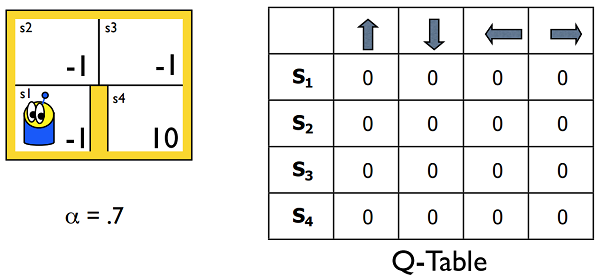
\includegraphics[width=.6\textwidth]{q_table}\end{center}
        
    \end{itemize}
\end{frame}

\begin{frame}{Q-learning and SARSA}
    \begin{itemize}
        \item Q-learning:\\
        \bigskip
        \hspace{0.5cm}\romannumeral2 . update $Q(s,a)$ with:\\
        \begin{equation}
            Q_{k+1}:=(1-\gamma_{k})Q_{k}+\gamma_{k}(r+\max\limits_{a' \in A}Q_{k}(s',a'))
        \end{equation}
        \hspace{0.7cm} where $\gamma_{k}$ is the learning rate, with $\sum_{k=1}^{\infty}\gamma_{k}=\infty$ and $\sum_{k=1}^{\infty}\gamma^2_{k}<\infty $ :\\
        \begin{equation}
            Q_{k+1}=Q_{k}+\gamma_{k}(r+\max\limits_{a' \in A}Q_{k}(s',a')-Q_{k}(s,a))
        \end{equation}
        \item Q-learning Demo: \href{https://www.google.com.hk}{google} \\
        
    \end{itemize}
\end{frame}

\begin{frame}{Q-learning and SARSA}
    \begin{itemize}
        \item Q-learning result:\\
    \end{itemize}
\end{frame}

\begin{frame}{Q-learning and SARSA}
    \begin{itemize}
        \item Exploration: $\epsilon - greedy$\\
        \begin{equation}
            a_{t}=\begin{cases}
             \arg\max_{a \in A}Q_{s_{t},a}, & \text{w.p.   } 1-\epsilon.\\
             unif(A), & \text{w.p.   } \epsilon.
        \end{cases}
        \end{equation}

        \item SARSA:\\
        \hspace{0.5cm}$\bullet$  update based on the current play $(s,a,r,s',a')$ \\
        \begin{equation}
            Q_{k+1}=Q_{k}+\gamma_{k}(r+Q_{k}(s',a')-Q_{k}(s,a))
        \end{equation}
        \hspace{0.5cm}$\bullet$  Similar to Q-learning but is On-policy \\


    \end{itemize}
\end{frame}



\begin{frame}{Deep Q-Networks}
    \begin{itemize}
         \item Drawback of Q-learning and SARSA:\\
         \bigskip
         \hspace{0.5cm}$\bullet$ Q-table can be too big if environment is complicate i.e. $1^6\times1^3$ maze\\
         \bigskip
         \item Alternative Algorithm: DQN:\\
         \bigskip
         \hspace{0.5cm}$\bullet$ Use a function approximator to estimate action-value function with Q-Network\\
         \bigskip
         \item Steps:\\
         \bigskip
         \hspace{0.5cm}$\romannumeral1$ store transition$(s_{t},s_{t},r_{t+1},s_{t+1})$ in memory\\
         \hspace{0.5cm}$\romannumeral2$ sample mini-batch of transitions, optimise MSE between Q-network and \\
         \hspace{0.7cm} Q-learning targets:\\
         \begin{equation}
            \text{minimize  }  L_{w}=E_{s,a,r,s'}[(r+\gamma \max\limits_{a'}Q(s',a';w^{-})-Q(s,a;w))^2]
        \end{equation}
        \hspace{0.5cm}$\romannumeral3$ 

    \end{itemize}
\end{frame}

\begin{frame}{Value Iteration: Problem}
    \begin{itemize}
        \item Recall: greedy action selection\\
        \begin{equation}
            \pi(s)=\arg\max\limits_{a' \in A}Q(s_{t+1},a')
        \end{equation}   
        \item Problem: deterministic, strategy fixed, not practical in Partially-Observed environment
    \end{itemize}
\end{frame}






\graphicspath{{./figs/repo/}{./figs/}}
\section{Optical Proximity Correction (OPC)}

\begin{frame}{Value Function Approximation}
    %{{{
    \begin{center}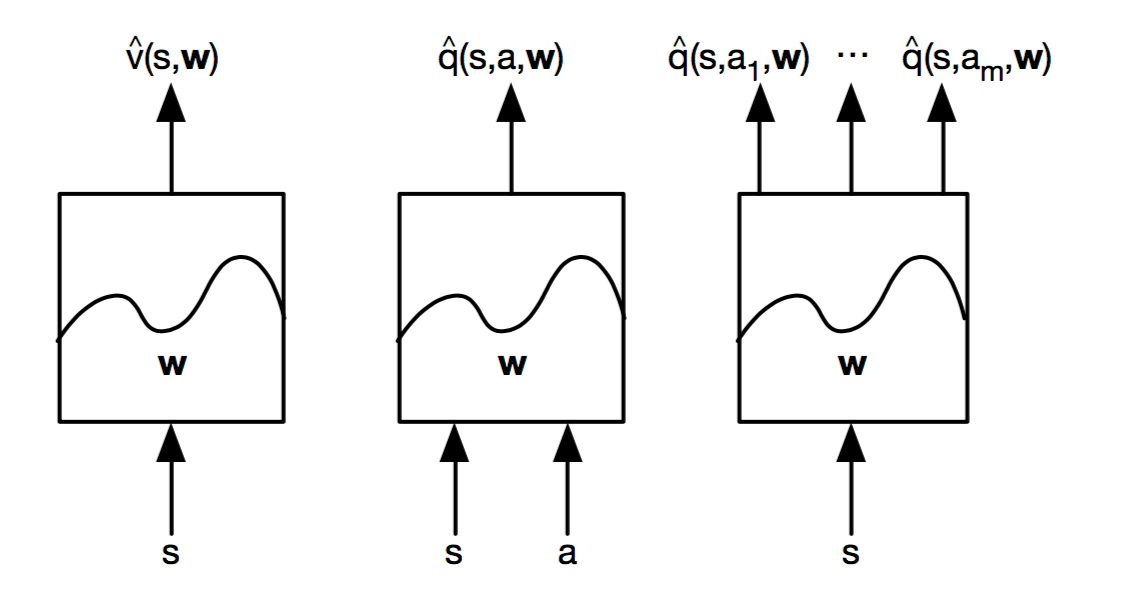
\includegraphics[width=.6\textwidth]{fun_app}\end{center}
    \begin{itemize}
        \item Tablular methods: impossible to record all states for real word problems 
        \item Function approximation: generalize from seen states to unseen states
    \end{itemize}
\end{frame}

\begin{frame}{Value Function Approximation}
    \begin{itemize}
        \item Goal: find parameter vector $w$ minimising mean-squared error between approximate value function $\hat{v}(S,w)$ and true value function $v_{\pi}(S)$
        \begin{align}
            \label{eq:1}
            J(w) = ||v_{\pi}(S)-\hat{v}(S,w)||_2^2
        \end{align}
        \item Stochastic gradient descent
        \begin{align}
            \label{eq:1}
            \Delta w = \alpha (v_{\pi}(s)-\hat{v}(S,w)) \nabla_{w}\hat{v}(S,w)
        \end{align}
        \item In reality we don't have the true value function $v_{\pi}(S)$\\
        \vspace{0.2cm}
        \hspace{0.5cm}$\bullet$ For Monte-Carlo, use discounted return $G_t$\\
        \vspace{0.2cm}
        \hspace{0.5cm}$\bullet$ For TD, use $R_{t+1}+\lambda \hat{v}(S_{t+1},w)$
        
    \end{itemize}
\end{frame}

\begin{frame}{Deep Q-Networks (DQN)}
    %{{{
    \begin{itemize}
        \item Take action $a_t$ according to $\epsilon$-greedy policy
        \item Store transition $(s_t,a_t,r_{t+1},s_{t+1})$ in memory $D$
        \item Sample random mini-batch of transitions $(s,a,r,s')$ from $D$
        \item Compute Q-learning targets w.r.t. old, fixed parameters $w^-$
        \item Optimise MSE between Q-network and Q-learning targets
            \begin{align}
                \label{eq:2}
                L(w) = \mathrm{E}_{s,a,s,r' \sim D_i}[(r+\gamma \max_{a'} Q(s',a';w^-)-Q(s,a;w))^2]
            \end{align}
        \item Two important tricks in ensuring convergence: experience replay and fixed target

    \end{itemize}
\end{frame}


\begin{frame}{Deep Q-Networks(DQN): play games in OpenAI gym}
    %{{{
    \begin{center}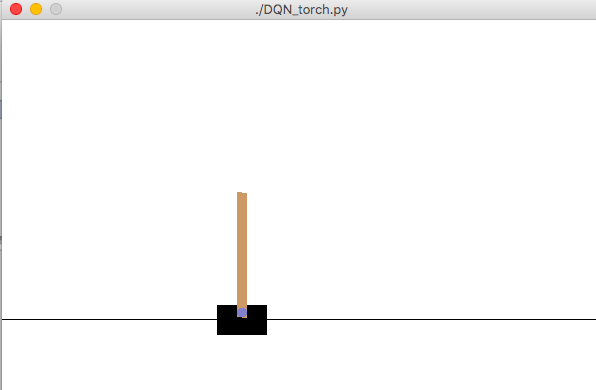
\includegraphics[width=.4\textwidth]{pole}\end{center}
    \begin{itemize}
        \item States are represented by 4-element tuples (position,cart velocity,angle,tip velocity)
        \item Actions can be either moving left or right
        \item Function approximator is a feed foward neural network 
        \item 1 hidden layer with 10 neurons, 2 output neurons representing value estimation for two actions
        \item Implemented using torch and tensorflow, can stay alive for 1 minute
    \end{itemize}

\end{frame}

\begin{frame}{Policy based method}
    Value based method (previous sildes):
    \begin{itemize}
        \item Main focus is on state-action value evaluation
        \item Policy improvement is based on greedy or $\epsilon$-greedy strategy w.r.t state-action values
        \item Return deterministic policy
    \end{itemize}\vspace{0.5cm}
    Policy based method (slides after this page):
    \begin{itemize}
        \item Policy is a function of observations
        \item Policy improvement is based on gradient w.r.t some objective function
        \item State-action value not neccessary for policy updates
        \item Return stochastic policy
    \end{itemize}
\end{frame}

\begin{frame}{Policy based method}
    What's wrong with value based methods?\\\vspace{0.2cm}
    \begin{center}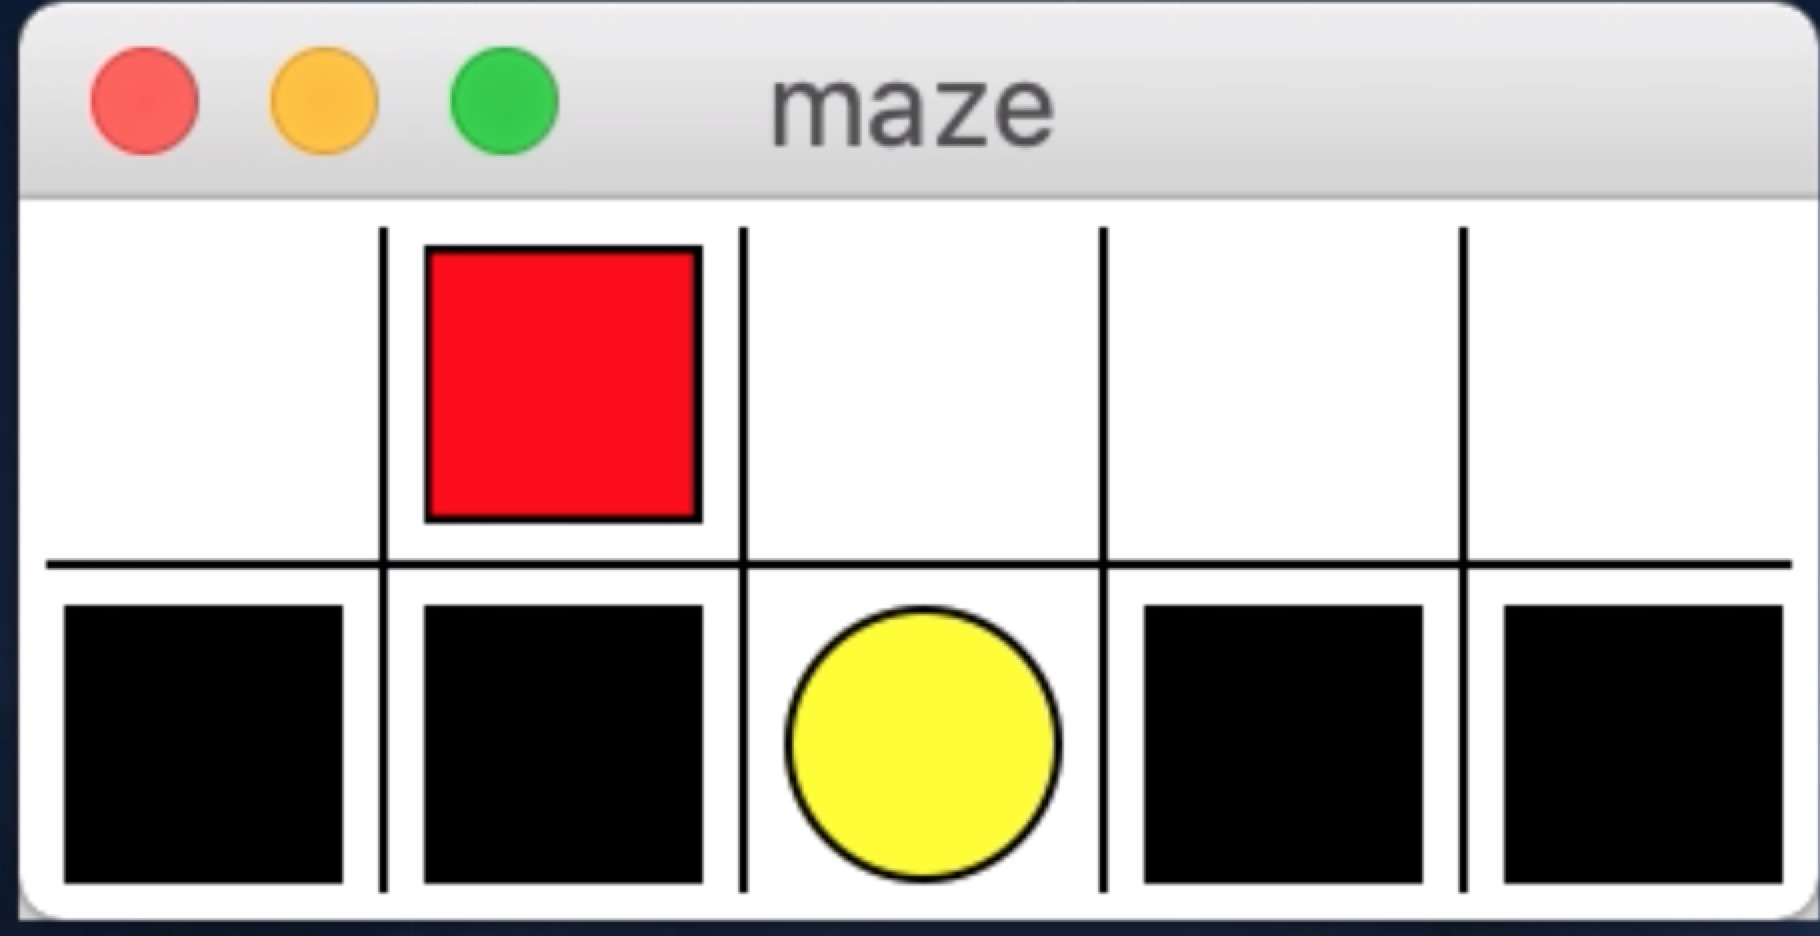
\includegraphics[width=.6\textwidth]{mirrorState}\end{center}
    \begin{itemize}
        \item Main problem: deterministic policy
        \item No good for partially observable environment
        \item Should I go left or right?
    \end{itemize}
\end{frame}

\begin{frame}{Policy Gradient: problem formulation}
    \begin{itemize}
        \item Policy is a function of observation: $\pi_{\theta}(\cdot)$\\\vspace{0.2cm}
        \item Trajectory $\tau$: $\{s_0,a_0,r_0,s_1,a_1,r_1,...\}$ is treated as random variable\\\vspace{0.2cm}
        \item Distribution of $\tau$ is determined by policy $\pi_{\theta}$\\\vspace{0.2cm}
        \item For each trajectory, total reward is defined as $R(\tau)$\\\vspace{0.2cm}
        \item Ultimate goal: optimize expectation $E_{\pi_{\theta}}[R(\tau)]$ w.r.t $\theta$\\\vspace{0.2cm}
    \end{itemize}
\end{frame}

\begin{frame}{Policy Gradient: approximate the gradient}
    \begin{itemize}
        \item What does the gradient look like?
        \begin{equation}
            \label{PG1}
            \begin{split}
            \nabla_\theta E_{\pi_{\theta}}[R(\tau)] &= \nabla_\theta \sum\limits_{\tau} P_\theta(\tau)R(\tau)\\ 
                                                &= \sum\limits_{\tau} \nabla_\theta P_\theta(\tau)R(\tau)\\
                                                &= \sum\limits_{\tau} P_\theta(\tau) \frac{\nabla_\theta P_\theta(\tau)}{P_\theta(\tau)} R(\tau) = E_{\pi_{\theta}}[\nabla_\theta\ln P_\theta(\tau)R(\tau)]\\
            \end{split}
        \end{equation}
        \item Equation \ref{PG1} tell us: gradient can be represented as an expectation\\\vspace{0.2cm}
        \item Why it is important: expectation can be approximated by sampling\\\vspace{0.2cm}
    \end{itemize}
\end{frame}

\begin{frame}{Policy Gradient: approximate the gradient}
    \begin{itemize}
        \item Why the gradient even exists?
            \begin{equation}
                \label{PG2}
                \begin{split}
                    P(\tau) = P(s_0) \prod\limits_{i=0}^\infty \pi_\theta(a_i,s_i) P(s_{i+1} | s_i,a_i)
                \end{split}
            \end{equation}
        \item Assumption: there is an underlying MDP specifying $P(s_{i+1} | s_i,a_i)$ and $P(s_0)$
            \begin{equation}
                \label{PG3}
                \begin{split}
                    \nabla_{\theta}\ln P(\tau) &= \nabla_{\theta}\ln [P(s_0) \prod\limits_{i=0}^\infty \pi_\theta(a_i,s_i) P(s_{i+1} | s_i,a_i)]\\
                                               &= \nabla_{\theta}\ln P(s_0) + \nabla_{\theta}\sum\limits_{i=0}^\infty [\ln \pi_\theta(a_i,s_i)+\ln P(s_{i+1} | s_i,a_i)]\\
                                               &= \nabla_{\theta}\sum\limits_{i=0}^\infty \ln \pi_\theta(a_i,s_i)
                \end{split}
            \end{equation}
    \end{itemize}
\end{frame}


\begin{frame}{Policy Gradient: understanding the formula}
    Combine all equation in previous slides, one important formula:
        \begin{equation}
            \label{PG4}
            \begin{split}
                \nabla_\theta E_{\pi_{\theta}}[R(\tau)] = E_{\pi_{\theta}}[R(\tau)\nabla_\theta\sum\limits_{s_i,a_i \in \tau}\ln\pi_\theta(a_i,s_i)]
            \end{split}
        \end{equation}
    Intuition from equation \ref{PG4}, adjustment magnitude of policy on $\pi_{\theta}(a,s)$:\vspace{0.2cm}
    \begin{itemize}
        \item In proportion to the total reward gained from trajectories containing $(a,s)$\vspace{0.2cm}
        \begin{itemize}
            \item Rationale: good actions lead to good trajectories, while bad actions lead to bad ones\vspace{0.2cm}
            \item What about good actions in trajectories with bad overall performance? work on it later\vspace{0.2cm}
        \end{itemize}\vspace{0.2cm}
        \item In inverse proportion to the probability of performing action $a$ on state $s$\vspace{0.2cm}
        \begin{itemize}
            \item consider actions sampled frequently but with small positive effect\vspace{0.2cm}
            \item mitigate case where 'not-so-good' actions are rewarded frequently\vspace{0.2cm}
        \end{itemize}
    \end{itemize}
\end{frame}


\begin{frame}{Vanilla Policy Gradient: \textbf{REINFORCE}}
    So far, we obtain the first policy gradient algotithm called \textbf{REINFORCE} \textcolor{CUHKgreen}{\footnotesize[Williams, R. J.]}
    \begin{center}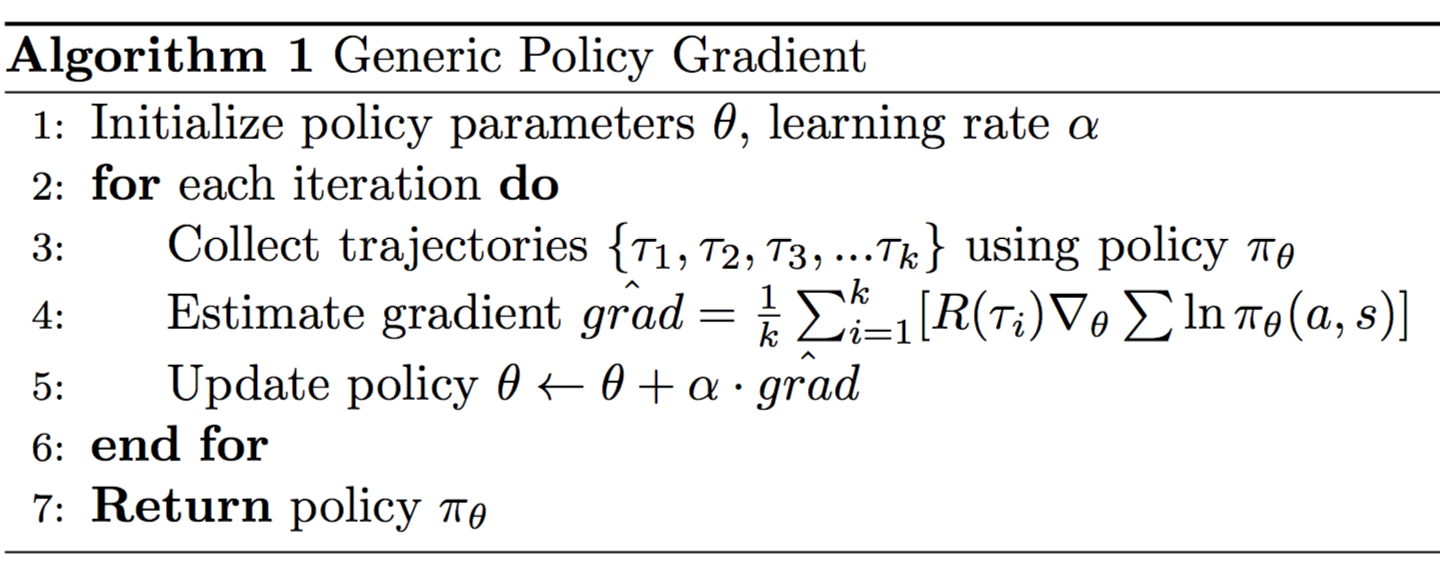
\includegraphics[width=.9\textwidth]{REINFORCE}\end{center}
\end{frame}

\begin{frame}{Vanilla Policy Gradient: \textbf{REINFORCE}}
    \vspace{0.2cm}
    \begin{center}Experiment on CartPole game:\\Bad performance, even not converge after 1000 episodes of training\\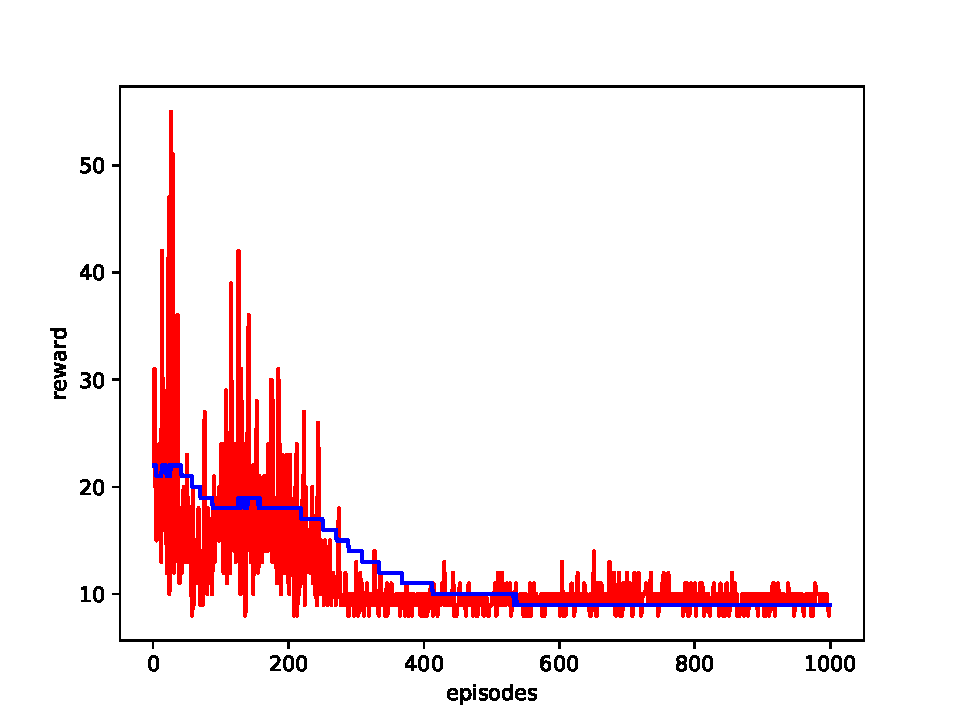
\includegraphics[width=.7\textwidth]{REINFORCE1}\end{center}
\end{frame}

\begin{frame}{Improvement for \textbf{REINFORCE}: baseline}
    \begin{itemize}
        \item One natural quetion: what if reward is always positive? \\
        \item Do we have to always increase $\pi_{\theta}(a,s)$ because $R(\tau)$ is positive (as in formula \ref{PG4})?\\
        \item Actually, we only cares about the relative performance of trajectories\\
        \item Observation from formula \ref{baseline}: we can remove any constant term $A$ from the expectation with out introducing bias.
        \item $A$ can be the average performance for all trajectories, it is referenced as a baseline
    \end{itemize}
    \begin{equation}
        \label{baseline}
        \begin{split}
            E_{\pi_\theta}[\sum\limits_{a}A\cdot\nabla\ln\pi(a,S)] &= \sum\limits_{a}\pi_\theta(a,S)A\frac{\nabla_\theta\pi_\theta(a,S)}{\pi_\theta(a,S)}\\
                                                                   &= A \sum\limits_{a}\nabla_\theta\pi(a,S)\\
                                                                   &= A\cdot\nabla_\theta\sum\limits_{a}\pi_\theta(a,S)= A \nabla_\theta(1)= 0
        \end{split}
    \end{equation}
    
\end{frame}

\begin{frame}{Improvement for \textbf{REINFORCE}: baseline}
    \vspace{0.2cm}
    \begin{center}Experiment on CartPole game:\\Better than before: an upgoing trend of rewards\\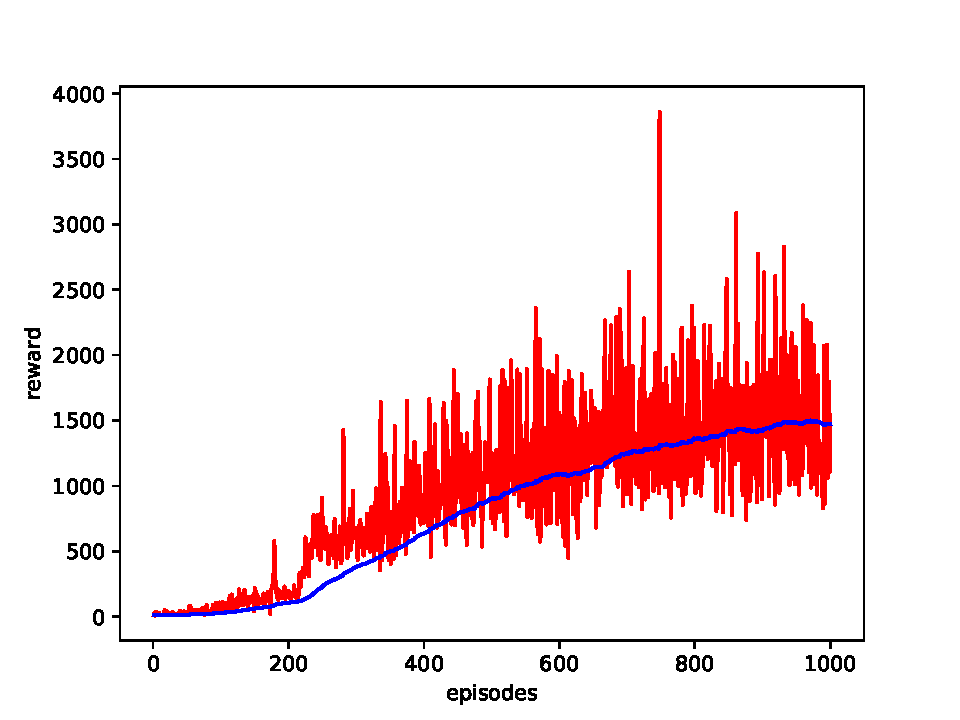
\includegraphics[width=.7\textwidth]{baseline_REINFORCE}\end{center}
\end{frame}

\begin{frame}{Improvement for \textbf{REINFORCE}: advantage function}
    \begin{itemize}
        \item Why we award/punish an action (s,a) based on the entire trajectory reward?\\
        \item Markov property: the action $a_t$ only affects rewards after time $t$.
        \begin{equation}
            \label{indp}
            \begin{split}
                E_{\pi_\theta}[R_{0:i-1}(\tau)\nabla_\theta\ln\pi_\theta(a_i,s_i)] = 0
            \end{split}
        \end{equation}  
        \item Actually, we can exploit the markov property to refine formula \ref{PG4}
            \begin{equation}
                    \label{refinePG1}
                    \begin{split}
                        \nabla_\theta E_{\pi_{\theta}}[R(\tau)] &=E_{\pi_{\theta}}[\sum(\nabla_\theta\ln\pi_\theta(a_i,s_i)(R_{0:i-1}(\tau)+R_{i:\infty}(\tau)))]\\
                        &=E_{\pi_{\theta}}[\sum(\nabla_\theta\ln\pi_\theta(a_i,s_i)R_{i:\infty}(\tau))]\\
                    \end{split}
            \end{equation}
        \item Recall that subtraction of baseline doesn't change the expectation
        \begin{equation}
                    \label{refinePG2}
                        \nabla_\theta E_{\pi_{\theta}}[R(\tau)] = E_{\pi_{\theta}}[\sum\nabla_\theta\ln\pi_\theta(a_i,s_i)(R_{i:\infty}(\tau)-V_{\pi_\theta}(s_i))]
        \end{equation}

    \end{itemize}  
\end{frame}

\begin{frame}{Improvement for \textbf{REINFORCE}: advantage function}
    \begin{itemize}
    \item As shown in equation \ref{refinePG2}, $R_{i:\infty}(\tau)-V_{\pi_\theta}(s_i)$ is the actual term that determines the magnitude we adjust probability $\pi_{\theta}(a_i,s_i)$\vspace{0.3cm}
    \item $R_{i:\infty}(\tau)-V_{\pi_\theta}(s_i)$ is also known as the advantage function \vspace{0.3cm}
    \item Rationale: extra reward gained when performing certain action $a_i$ on state $s_i$ compared to average reward from that state under policy $\pi_{\theta}$\vspace{0.3cm}
    \end{itemize}
\end{frame}

\begin{frame}{Improvement for \textbf{REINFORCE}: advantage function}
    \vspace{0.2cm}
    \begin{center}Experiment on CartPole game:\\Only after 141 episodes of training, surviving time boosted to 20k! \\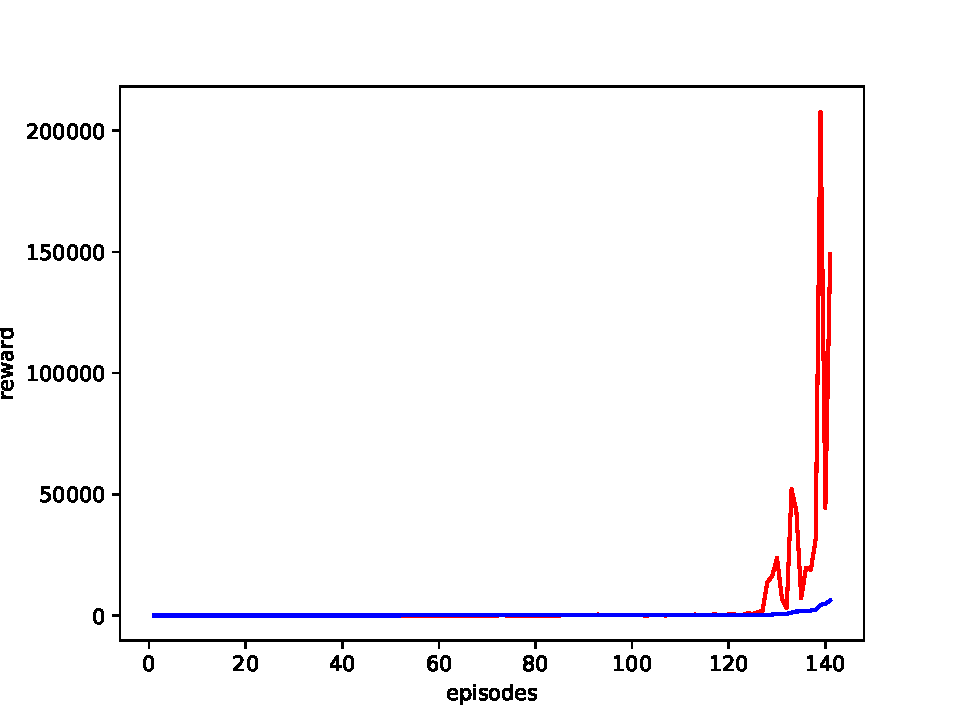
\includegraphics[width=.7\textwidth]{adv_REINFORCE}\end{center}
\end{frame}

\begin{frame}{Actor-Critic: a combination}
    So far, we mainly focused on pure value-based and pure policy-based methods ... \vspace{0.3cm}
    \begin{itemize}
        \item Value-based: problem of deterministic policy in partially observed environments\vspace{0.3cm}
        \item Policy-based: credit assignment problem (delay between action and reward)\vspace{0.3cm}
        \item Why not combine them?\vspace{0.3cm}
        \item Still use parameterized function for policy\vspace{0.3cm}
        \item But also add an estimator for state values to approximate advantage function\vspace{0.3cm}
        \item Stochastic policy agent without problem of update delay!
    \end{itemize}
\end{frame}

\begin{frame}{Actor-Critic: algorithm}
    \vspace{0.2cm}
    Now there are two function to learn: policy function $\pi_{\theta}$ is known as actor and value estimator $\hat{V_{\varphi}}$ is known as critic, hence the model named \textbf{Actor-Critic}.\\\vspace{0.2cm}
    The overall algorithm can be like this (there are many variants, this is what we use in our experiment)\\\vspace{0.2cm}
    \begin{center}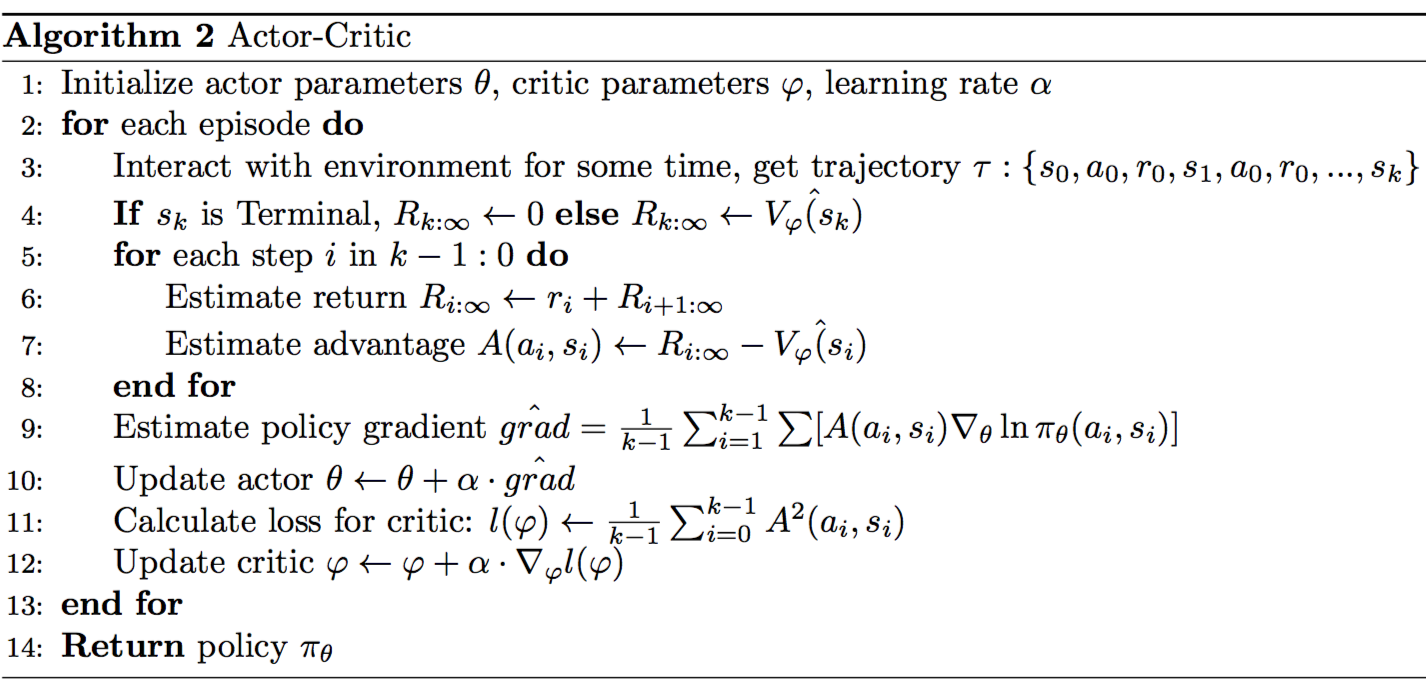
\includegraphics[width=.8\textwidth]{AC1}\end{center}
\end{frame}

\begin{frame}{Further improvement: clipped objective function}
    \begin{itemize}
        \item In previous section, policy gradient method works by computing gradient estimator in form
            \begin{equation}
                \label{commonPG}
                \hat{g} = \hat{E_t}[\nabla_{\theta}\ln\pi_\theta(a_t,s_t)\hat{A}_{t}]
            \end{equation}
        \item The estimator $\hat{g}$ can be obtained by differentiating the objective
            \begin{equation}
                \label{objPG}
                L^{PG}(\theta) = \hat{E_t}[\ln\pi_\theta(a_t,s_t)\hat{A}_{t}]
            \end{equation}
        \item Multiple steps to optimize $L^{PG}$ on same trajectory: destructively large policy updates \textcolor{CUHKgreen}{\footnotesize[Schulman, John et al.]}. 
        \item To improve sample efficiency, they adopt strategy of clipping the surrogate objective function in form $L^{CPI}(\theta)$:

    \end{itemize} 
\end{frame}

\begin{frame}{Further improvement: clipped objective function}
\begin{equation}
                \label{objPPO}
                L^{CPI}(\theta) = \hat{E_t}[\frac{\pi_\theta(a_t,s_t)}{\pi_{\theta_{old}}(a_t,s_t)}\hat{A}_{t}]
            \end{equation}
\begin{itemize}
    \item $\pi_{\theta_{old}}$: fixed term generated by old policy\vspace{0.2cm}
    \item $\pi_{\theta}$: current policy being optimized. \vspace{0.2cm}
    \item The ratio $\frac{\pi_\theta(a_t,s_t)}{\pi_{\theta_{old}}(a_t,s_t)}$ is denoted as $r_t(\theta)$\vspace{0.2cm}
    \item $r_t(\theta)$ measures the difference between current policy and old policy\vspace{0.2cm}
    \item we don't want too big a update step, hence some constraint based on $r_t(\theta)$\vspace{0.2cm}
    \item In practise we use the gradient of following objective function\vspace{0.2cm}
\end{itemize}
\begin{equation}
    \label{clipPPO}
    L^{CLIP}(\theta) = \hat{E_t}[\min(r_t(\theta)\hat{A_t},\mathrm{clip}(r_t(\theta),1-\epsilon,1+\epsilon)\hat{A_t}]
\end{equation}
\end{frame}

\begin{frame}{Further improvement: clipped objective function}
    \vspace{0.15cm}
    The algorithm is known as Proximal Policy Optimization \textcolor{CUHKgreen}{\footnotesize[Schulman, John et al.]}\\\vspace{0.15cm}
    Only with minor modification on previous Actor-Critic algorithm:\\\vspace{0.1cm}
    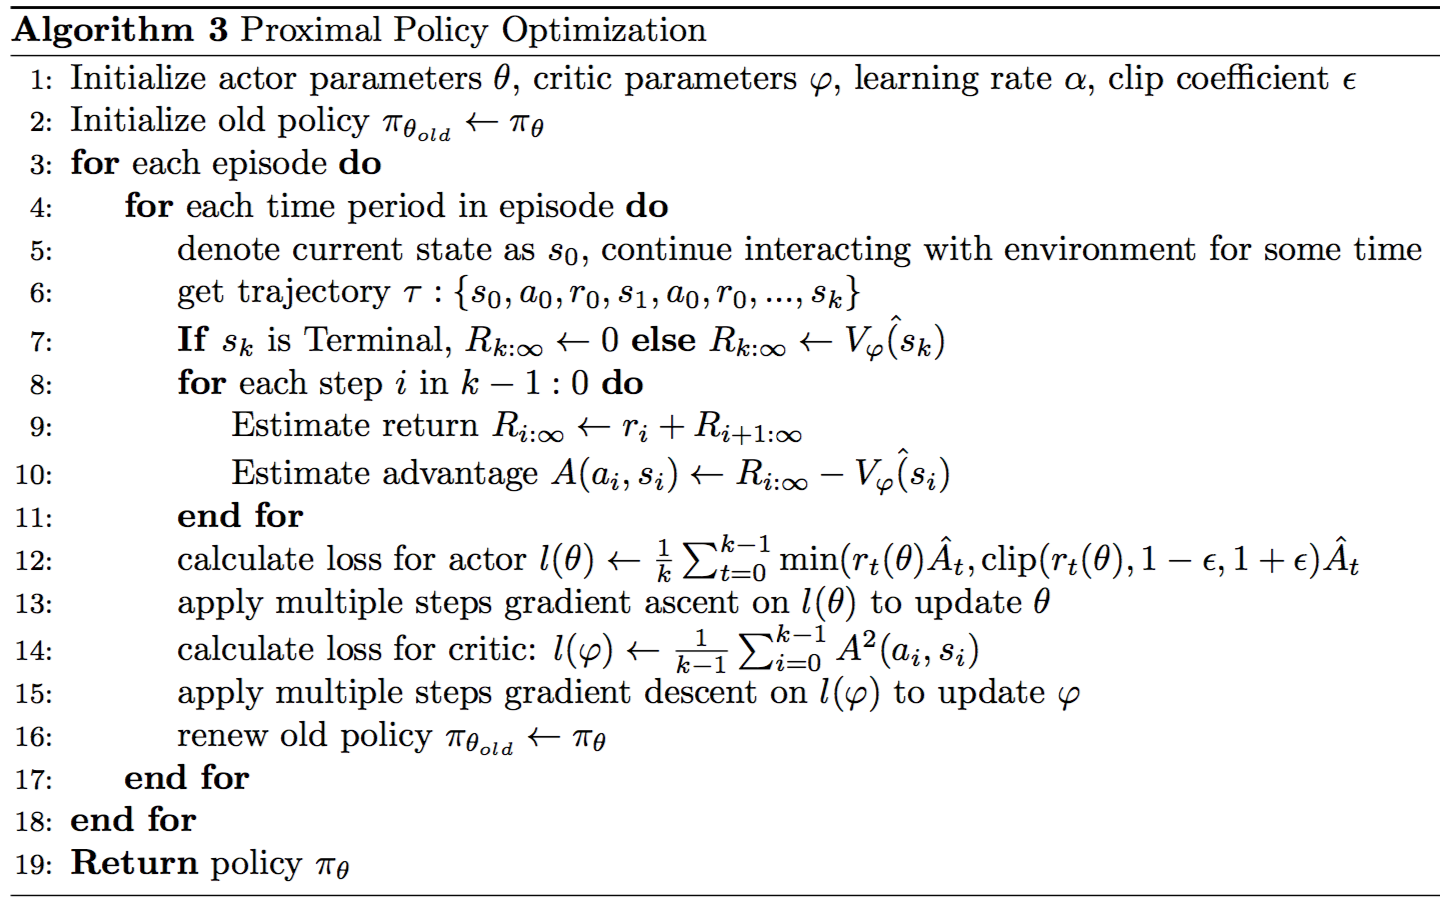
\includegraphics[width=.8\textwidth]{PPO1}
\end{frame}

\begin{frame}{Further improvement: high score buffer replay}
    
    
\end{frame}


\end{document}

